% !TeX program = xelatex
\documentclass[a4paper,10pt]{article}

% ============================================================================
% កញ្ចប់បណ្ណាល័យ (Packages) – តាមលំនាំ NGS Preah Krasang (ls_plan.tex)
% ============================================================================
\usepackage[a4paper, left=0.95cm, right=0.95cm, top=0.80cm, bottom=1.06cm, footskip=0.58cm]{geometry}
\usepackage{amsmath, amssymb}
\usepackage{unicode-math}
\usepackage{fontspec}
\usepackage{array, longtable, multirow, colortbl}
\usepackage[table]{xcolor}
\usepackage{enumitem}
\usepackage{pifont}
\usepackage{fancyhdr}
\usepackage{tikz}
\usetikzlibrary{calc, arrows.meta, angles, quotes, decorations.markings, decorations.pathreplacing, patterns, babel}

% LaTeX 2025 + longtable v4.24 compatibility guard
\makeatletter
\let\@expl@@@mark@update@singlecol@structures@@\relax
\makeatother

% ============================================================================
% ការកំណត់ពុម្ពអក្សរ (Fonts Configuration - Cross-Platform Windows + Cloud fonts/)
% ============================================================================
\providecommand{\NGSFindFonts}{%
  \IfFileExists{C:/Windows/Fonts/cambria.ttc}{%
    \def\NGSSysPath{C:/Windows/Fonts/}%
    \def\NGSUserPath{C:/Users/KIT/AppData/Local/Microsoft/Windows/Fonts/}%
  }{%
    \IfFileExists{./fonts/KhmerOSsiemreap.ttf}{\def\NGSSysPath{./fonts/}\def\NGSUserPath{./fonts/}}{%
    \IfFileExists{../fonts/KhmerOSsiemreap.ttf}{\def\NGSSysPath{../fonts/}\def\NGSUserPath{../fonts/}}{%
    \IfFileExists{../../fonts/KhmerOSsiemreap.ttf}{\def\NGSSysPath{../../fonts/}\def\NGSUserPath{../../fonts/}}{%
    \IfFileExists{../../../fonts/KhmerOSsiemreap.ttf}{\def\NGSSysPath{../../../fonts/}\def\NGSUserPath{../../../fonts/}}{%
    \IfFileExists{../../../../fonts/KhmerOSsiemreap.ttf}{\def\NGSSysPath{../../../../fonts/}\def\NGSUserPath{../../../../fonts/}}{%
    \IfFileExists{../../../../../fonts/KhmerOSsiemreap.ttf}{\def\NGSSysPath{../../../../../fonts/}\def\NGSUserPath{../../../../../fonts/}}{%
    \IfFileExists{../../../../../../fonts/KhmerOSsiemreap.ttf}{\def\NGSSysPath{../../../../../../fonts/}\def\NGSUserPath{../../../../../../fonts/}}{%
      \def\NGSSysPath{../../../../../../../fonts/}\def\NGSUserPath{../../../../../../../fonts/}%
    }}}}}}}%
  }%
}
\NGSFindFonts

\setmathfont[
  Path={\NGSSysPath},
  FontIndex=1,
  Scale=1.02
]{cambria.ttc}

\defaultfontfeatures{Ligatures=TeX}

\setmainfont[
  Path={\NGSUserPath},
  Extension=.ttf,
  Script=Khmer,
  BoldFont={KhmerOSsiemreap},
  BoldFeatures={FakeBold=1.8},
  ItalicFont={KhmerOSsiemreap},
  ItalicFeatures={FakeSlant=0.25},
  BoldItalicFont={KhmerOSsiemreap},
  BoldItalicFeatures={FakeBold=1.8, FakeSlant=0.25}
]{KhmerOSsiemreap}

\newfontfamily\muol[
  Path={\NGSUserPath},
  Extension=.ttf,
  Script=Khmer
]{KhmerOSmuollight}

\newfontfamily\TimesEn[
  Path={\NGSSysPath},
  Extension=.ttf,
  Scale=1.00,
  BoldFont={timesbd},
  ItalicFont={timesi},
  BoldItalicFont={timesbi}
]{times}

\newfontfamily\NagaBold[
  Path={\NGSUserPath},
  Extension=.ttf
]{AKbalthom Naga Bold}

\newfontfamily\CalibriFont[
  Path={\NGSSysPath},
  Extension=.ttf
]{calibri}

\newfontfamily\Tacteing[
  Path={\NGSUserPath}
]{TACTENG.TTF}

\newfontfamily\CourierBullet[
  Path={\NGSSysPath},
  Extension=.ttf
]{cour}
\newcommand{\wcirc}{{\CourierBullet\fontsize{9.5pt}{11pt}\selectfont o}}

% ក្បួនកាត់ពាក្យខ្មែរ (Khmer word wrapping)
\XeTeXlinebreaklocale "km"
\XeTeXlinebreakskip = 0pt plus 1pt minus 0.1pt

% ============================================================================
% ការកំណត់ពណ៌ និងទម្រង់ទំព័រ (Colors & Page Style)
% ============================================================================
\definecolor{stepgray}{HTML}{D9D9D9}
\definecolor{headgray}{HTML}{F2F2F2}
\definecolor{boxgray}{HTML}{D9D9D9}
\definecolor{darkred}{HTML}{C00000}
\definecolor{red5e}{HTML}{FF0000}

\pagestyle{fancy}
\fancyhf{}
\renewcommand{\headrulewidth}{0pt}
\fancyfoot[R]{\CalibriFont\fontsize{11pt}{13pt}\selectfont\thepage}

\setlength{\parindent}{0pt}
\setlength{\parskip}{0pt}
\setlength{\tabcolsep}{3.8pt}

\newcolumntype{L}[1]{>{\raggedright\arraybackslash}p{#1}}

% ============================================================================
% ម៉ាក្រូជំនួយ (Helper Macros)
% ============================================================================
\newcommand{\en}[1]{{\TimesEn #1}}
\newcommand{\enbf}[1]{{\TimesEn\textbf{#1}}}
\newcommand{\unit}[1]{\,\text{\en{#1}}}
\newcommand{\fiveE}[1]{{\NagaBold\fontsize{9.5pt}{13pt}\selectfont\textcolor{red5e}{#1}}}
\newcommand{\timenote}[1]{\textcolor{darkred}{\textit{#1}}}
\newcommand{\redsub}[1]{\textcolor{darkred}{#1}}
\newcommand{\graybox}[1]{\colorbox{boxgray}{\strut\hspace{2pt}#1\hspace{2pt}}}
\newcommand{\ditem}{\tikz[baseline=-0.5ex]\fill (0,0.42ex) -- (0.42ex,0) -- (0,-0.42ex) -- (-0.42ex,0) -- cycle;\hspace{0.3em}}
\newcommand{\cnum}[1]{{\fontsize{10.5pt}{12pt}\selectfont\ding{\numexpr181+#1\relax}}\hspace{0.15em}}
\newcommand{\cfig}[1]{\par\vspace{2pt}{\centering #1\par}\vspace{2pt}}
\newcommand{\stepheader}[1]{\multicolumn{3}{|c|}{\cellcolor{stepgray}\muol #1} \\* \noalign{\hrule height 0.4pt}}
\newcommand{\circbox}[1]{\tikz[baseline=(c.base)]\node[draw=black, rounded corners=3.5pt, line width=0.8pt, inner sep=1.3pt] (c) {\ensuremath{#1}};}

% ក្បាច់ក្រោមបាវចនា (Tacteing Font - Keyboard '3')
\newcommand{\khmflourish}{{\Tacteing\fontsize{36pt}{14pt}\selectfont\raisebox{-5pt}{3}}}

% ============================================================================
% ម៉ាក្រូគូសរូប TikZ ស-ខ្មៅ ១០០% (Monochrome B&W, Black Labels >= 8.5pt, 6.2-7.1cm)
% ============================================================================

% ១. ជំហានទី២ កំណែ ២.១ និងស្ពានគោល ១០ ភ្ជាប់និទស្សន្ត ០/អវិជ្ជមាន (2 wide stacked panels)
\newcommand{\figStepTwoReviewEXP}{%
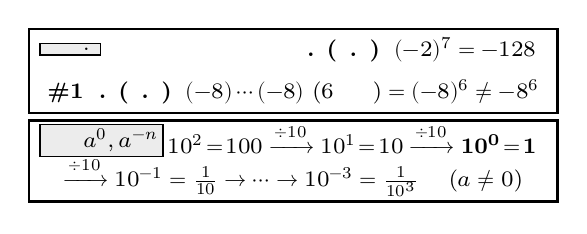
\begin{tikzpicture}[scale=0.92, every node/.style={font=\footnotesize, text=black}]
  % លើ៖ កំណែ ២.១ ប្រយ័ត្នវង់ក្រចក
  \draw[black, line width=0.95pt] (0,1.22) rectangle (7.30,2.38);
  \node[anchor=west, fill=gray!15, draw=black, line width=0.6pt, inner sep=1.6pt] at (0.14,2.10) {កំណែ ២.១};
  \node[anchor=east] at (7.14,2.10) {\textbf{ប្រតិបត្តិ ២ គ. (ទំ.១៤)៖} $(-2)^7 = -128$};
  \node at (3.65,1.52) {\textbf{\#1 ខ. (ទំ.២៥)៖} $(-8)\cdots(-8)\text{ ($6$ កត្តា)} = (-8)^6 \neq -8^6$};

  % ក្រោម៖ លំនាំស្វ័យគុណគោល ១០ (ចែក ១០)
  \draw[black, line width=0.95pt] (0,0) rectangle (7.30,1.12);
  \node[anchor=west, fill=gray!15, draw=black, line width=0.6pt, inner sep=1.6pt] at (0.14,0.84) {ស្ពាន $a^0, a^{-n}$};
  \node[anchor=east] at (7.14,0.84) {$10^2\!=\!100 \xrightarrow{\div 10} 10^1\!=\!10 \xrightarrow{\div 10} \mathbf{10^0\!=\!1}$};
  \node at (3.65,0.32) {$\xrightarrow{\div 10} 10^{-1}=\tfrac{1}{10} \to\cdots\to 10^{-3}=\tfrac{1}{10^3}$ \quad ($a\neq 0$)};
\end{tikzpicture}}

% ២. E1 Engage: បេសកកម្មឃ្លាំងវីដេអូ Server បណ្ណាល័យឌីជីថលព្រះក្រសាំង (2 wide stacked panels)
\newcommand{\figEngageServerEXP}{%
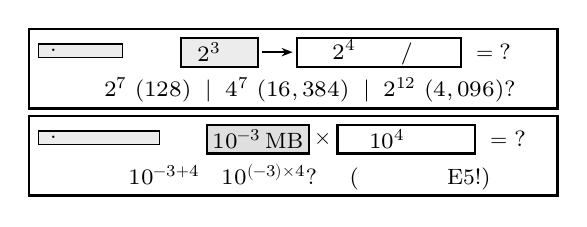
\begin{tikzpicture}[scale=0.92, every node/.style={font=\footnotesize, text=black}]
  % លើ៖ 2^3 ថត x 2^4 វីដេអូ
  \draw[black, line width=0.95pt] (0,1.20) rectangle (7.30,2.30);
  \node[anchor=west, fill=gray!15, draw=black, line width=0.6pt, inner sep=2pt] at (0.12,2.00) {ក. ថតវីដេអូ};
  \draw[black, line width=0.8pt, fill=gray!15] (2.10,1.78) rectangle (3.16,2.18);
  \node at (2.63,1.98) {$2^3$ ថត};
  \draw[black, line width=0.8pt, -{Stealth[length=4pt]}] (3.22,1.98) -- (3.64,1.98);
  \draw[black, line width=0.8pt, fill=white] (3.70,1.78) rectangle (5.96,2.18);
  \node at (4.83,1.98) {$2^4$ វីដេអូ/ថត};
  \node[anchor=west] at (6.04,1.98) {$= ?$};
  \node at (3.65,1.46) {\textbf{ទាយ៖} $2^7$ ($128$) \;\textbar{}\; $4^7$ ($16,384$) \;\textbar{}\; $2^{12}$ ($4,096$)?};

  % ក្រោម៖ កញ្ចប់បង្ហាប់ទិន្នន័យ 10^-3 x 10^4 MB
  \draw[black, line width=0.95pt] (0,0) rectangle (7.30,1.10);
  \node[anchor=west, fill=gray!15, draw=black, line width=0.6pt, inner sep=2pt] at (0.12,0.80) {ខ. កញ្ចប់ទិន្នន័យ};
  \draw[black, line width=0.8pt, fill=gray!25] (2.46,0.58) rectangle (3.86,0.98);
  \node at (3.16,0.78) {$10^{-3}\unit{MB}$};
  \node at (4.06,0.78) {$\times$};
  \draw[black, line width=0.8pt, fill=white] (4.26,0.58) rectangle (6.16,0.98);
  \node at (5.21,0.78) {$10^4$ ឯកសារ};
  \node[anchor=west] at (6.24,0.78) {$= ?$};
  \node at (3.65,0.26) {\textbf{ទាយ៖} $10^{-3+4}$ ឬ $10^{(-3)\times 4}$? \quad (កត់ទុកផ្ទៀងនៅ \en{E5}!)};
\end{tikzpicture}}

% ៣. E2 Act 1A: បន្ទះកត្តា 1:1 (2^3 = 3cm + 2^4 = 4cm -> 7cm = 2^7)
\newcommand{\figExploreStripsEXP}{%
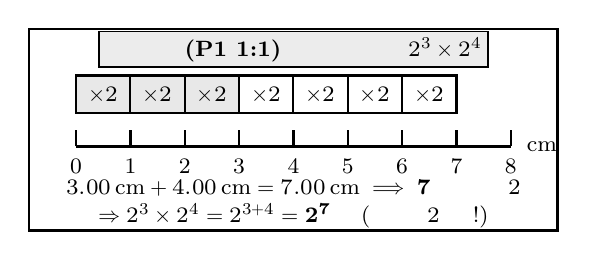
\begin{tikzpicture}[scale=0.92, every node/.style={font=\footnotesize, text=black}]
  \draw[black, line width=0.95pt] (0,0) rectangle (7.30,2.78);
  \node[fill=gray!15, draw=black, line width=0.6pt, inner sep=2pt] at (3.65,2.50) {\textbf{សកម្មភាព ១ក (\en{P1 1:1})៖} តភ្ជាប់បន្ទះកត្តា $2^3 \times 2^4$};

  % Strip 2^3 (3 units) + Strip 2^4 (4 units) concatenated on 0-8 track
  \draw[black, line width=1.0pt, fill=gray!18] (0.65,1.62) rectangle (2.90,2.14);
  \draw[black, line width=0.75pt] (1.40,1.62)--(1.40,2.14) (2.15,1.62)--(2.15,2.14);
  \node at (1.025,1.88) {$\times 2$};
  \node at (1.775,1.88) {$\times 2$};
  \node at (2.525,1.88) {$\times 2$};

  \draw[black, line width=1.0pt, fill=white] (2.90,1.62) rectangle (5.90,2.14);
  \draw[black, line width=0.75pt] (3.65,1.62)--(3.65,2.14) (4.40,1.62)--(4.40,2.14) (5.15,1.62)--(5.15,2.14);
  \node at (3.275,1.88) {$\times 2$};
  \node at (4.025,1.88) {$\times 2$};
  \node at (4.775,1.88) {$\times 2$};
  \node at (5.525,1.88) {$\times 2$};

  % Ruler ticks below (0 to 8 cm)
  \draw[black, line width=0.9pt] (0.65,1.16) -- (6.65,1.16);
  \foreach \k in {0,...,8}{
    \pgfmathsetmacro{\kx}{0.65 + \k*0.75}
    \draw[black, line width=0.8pt] (\kx,1.16) -- (\kx,1.38);
    \node[below=1pt] at (\kx,1.16) {\en{\k}};
  }
  \node[right=1.5pt] at (6.68,1.16) {\en{cm}};

  % Bottom synthesis
  \node at (3.65,0.58) {$3.00\unit{cm} + 4.00\unit{cm} = 7.00\unit{cm} \implies \mathbf{7}$ កត្តាគុណនៃ $2$};
  \node at (3.65,0.20) {$\Rightarrow 2^3 \times 2^4 = 2^{3+4} = \mathbf{2^7}$ \quad (រក្សាគោល $2$ ដដែល!)};
\end{tikzpicture}}

% ៤. E2 Act 1B: ផ្ទាំងបន្សាបគូសូន្យ 1:1 (10^-3 x 10^4 = 10^1)
\newcommand{\figExploreZeroPairEXP}{%
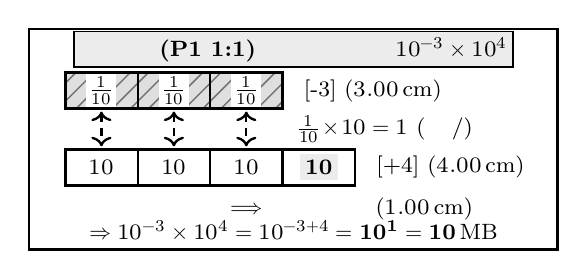
\begin{tikzpicture}[scale=0.92, every node/.style={font=\footnotesize, text=black}]
  \draw[black, line width=0.95pt] (0,-0.06) rectangle (7.30,2.98);
  \node[fill=gray!15, draw=black, line width=0.6pt, inner sep=2pt] at (3.65,2.70) {\textbf{សកម្មភាព ១ខ (\en{P1 1:1})៖} ផ្ទាំងបន្សាបគូសូន្យ $10^{-3} \times 10^4$};

  % Hatched [-3] strip: 3 cells of 1/10
  \draw[black, line width=1.0pt, fill=gray!25] (0.50,1.88) rectangle (3.50,2.38);
  \begin{scope}
    \clip (0.50,1.88) rectangle (3.50,2.38);
    \foreach \hx in {0.15, 0.40, ..., 3.75}{
      \draw[black!55, line width=0.55pt] (\hx,1.88) -- (\hx+0.50,2.38);
    }
  \end{scope}
  \draw[black, line width=1.0pt] (0.50,1.88) rectangle (3.50,2.38);
  \draw[black, line width=0.8pt] (1.50,1.88)--(1.50,2.38) (2.50,1.88)--(2.50,2.38);
  \node[fill=white, inner sep=0.8pt] at (1.00,2.13) {$\frac{1}{10}$};
  \node[fill=white, inner sep=0.8pt] at (2.00,2.13) {$\frac{1}{10}$};
  \node[fill=white, inner sep=0.8pt] at (3.00,2.13) {$\frac{1}{10}$};
  \node[anchor=west] at (3.66,2.13) {\en{[-3]} ($3.00\unit{cm}$)};

  % 3 dashed 1-to-1 cancellation arrows
  \foreach \px in {1.00, 2.00, 3.00}{
    \draw[black, densely dashed, line width=0.85pt, <->] (\px,1.84) -- (\px,1.36);
  }
  \node[anchor=west] at (3.55,1.60) {$\frac{1}{10}\!\times\!10 = 1$ (គូស \en{/})};

  % Solid [+4] strip: 4 cells of 10
  \draw[black, line width=1.0pt, fill=white] (0.50,0.82) rectangle (4.50,1.32);
  \draw[black, line width=0.8pt] (1.50,0.82)--(1.50,1.32) (2.50,0.82)--(2.50,1.32) (3.50,0.82)--(3.50,1.32);
  \node at (1.00,1.07) {$10$};
  \node at (2.00,1.07) {$10$};
  \node at (3.00,1.07) {$10$};
  \node[fill=gray!15, inner sep=2pt] at (4.00,1.07) {\textbf{10}};
  \node[anchor=west] at (4.66,1.07) {\en{[+4]} ($4.00\unit{cm}$)};

  % Bottom synthesis
  \node at (3.65,0.50) {បន្សាប ៣ គូសូន្យ $\implies$ នៅសល់ \textbf{១ ប្រអប់} ($1.00\unit{cm}$)};
  \node at (3.65,0.20) {$\Rightarrow 10^{-3} \times 10^4 = 10^{-3+4} = \mathbf{10^1 = 10\unit{MB}}$};
\end{tikzpicture}}

% ៥. E2 Act 2A: Dual POE 2A (អន្ទាក់គុណគោល និងគោលខុសគ្នា + រូបប្លុកបង្វិល 25°)
\newcommand{\figExplorePOETwoAEXP}{%
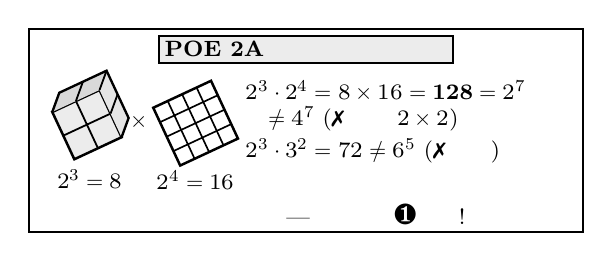
\begin{tikzpicture}[scale=0.92, every node/.style={font=\footnotesize, text=black}]
  \draw[black, line width=0.95pt] (0,0) rectangle (7.65,2.80);
  \node[fill=gray!15, draw=black, line width=0.6pt, inner sep=2pt] at (3.825,2.52) {\textbf{\en{POE 2A}៖} អន្ទាក់គុណគោល និងគោលខុសគ្នា};

  % Rotated ~25 deg 2x2x2 cube (2^3 = 8)
  \begin{scope}[shift={(0.80,1.48)}, rotate=25]
    \fill[gray!15] (-0.36,-0.36) rectangle (0.36,0.36);
    \draw[black, line width=0.9pt] (-0.36,-0.36) rectangle (0.36,0.36);
    \draw[black, line width=0.65pt] (0,-0.36)--(0,0.36) (-0.36,0)--(0.36,0);
    \fill[gray!30] (-0.36,0.36)--(0.36,0.36)--(0.56,0.56)--(-0.16,0.56)--cycle;
    \fill[gray!20] (0.36,-0.36)--(0.56,-0.16)--(0.56,0.56)--(0.36,0.36)--cycle;
    \draw[black, line width=0.85pt] (-0.36,0.36)--(-0.16,0.56)--(0.56,0.56)--(0.56,-0.16)--(0.36,-0.36);
    \draw[black, line width=0.65pt] (0.36,0.36)--(0.56,0.56) (0,0.36)--(0.20,0.56) (0.36,0)--(0.56,0.20);
  \end{scope}
  \node at (0.84,0.72) {$2^3 = 8$};

  \node at (1.52,1.52) {$\times$};

  % Rotated ~25 deg 4x4 grid (2^4 = 16)
  \begin{scope}[shift={(2.30,1.50)}, rotate=25]
    \fill[white] (-0.44,-0.44) rectangle (0.44,0.44);
    \draw[black, line width=0.9pt] (-0.44,-0.44) rectangle (0.44,0.44);
    \foreach \g in {-0.22, 0, 0.22}{
      \draw[black, line width=0.6pt] (\g,-0.44)--(\g,0.44) (-0.44,\g)--(0.44,\g);
    }
  \end{scope}
  \node at (2.30,0.72) {$2^4 = 16$};

  % Comparison math on right (concise, comfortable right margin inside 7.65)
  \node[anchor=west, align=left] at (2.86,1.52)
    {$2^3\cdot 2^4 = 8\times 16 = \mathbf{128} = 2^7$\\
     $\quad \neq 4^7$ (\ding{55} គុណគោល $2\times 2$)\\[2pt]
     $2^3\cdot 3^2 = 72 \neq 6^5$ (\ding{55} ខុសគោល)};

  \node at (3.825,0.24) {\textbf{សន្និដ្ឋាន៖} ហាមគុណគោល — ពិនិត្យច្រក \cnum{1} ជាមុន!};
\end{tikzpicture}}

% ៦. E2 Act 2B: Dual POE 2B (គុណនិទស្សន្ត & ភ្លេចនិទស្សន្តលាក់ 1 + រូបប្លុកបង្វិល 25°)
\newcommand{\figExplorePOETwoBEXP}{%
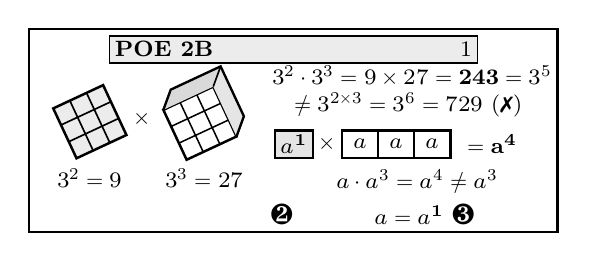
\begin{tikzpicture}[scale=0.92, every node/.style={font=\footnotesize, text=black}]
  \draw[black, line width=0.95pt] (0,0) rectangle (7.30,2.80);
  \node[fill=gray!15, draw=black, line width=0.6pt, inner sep=2pt] at (3.65,2.52) {\textbf{\en{POE 2B}៖} អន្ទាក់គុណនិទស្សន្ត និងនិទស្សន្តលាក់ \en{1}};

  % Rotated ~25 deg 3x3 grid (3^2 = 9)
  \begin{scope}[shift={(0.84,1.52)}, rotate=25]
    \fill[gray!15] (-0.38,-0.38) rectangle (0.38,0.38);
    \draw[black, line width=0.9pt] (-0.38,-0.38) rectangle (0.38,0.38);
    \draw[black, line width=0.6pt] (-0.127,-0.38)--(-0.127,0.38) (0.127,-0.38)--(0.127,0.38);
    \draw[black, line width=0.6pt] (-0.38,-0.127)--(0.38,-0.127) (-0.38,0.127)--(0.38,0.127);
  \end{scope}
  \node at (0.84,0.74) {$3^2=9$};

  \node at (1.56,1.56) {$\times$};

  % Rotated ~25 deg 3x3x3 cube (3^3 = 27)
  \begin{scope}[shift={(2.36,1.50)}, rotate=25]
    \fill[white] (-0.38,-0.38) rectangle (0.38,0.38);
    \draw[black, line width=0.9pt] (-0.38,-0.38) rectangle (0.38,0.38);
    \draw[black, line width=0.55pt] (-0.127,-0.38)--(-0.127,0.38) (0.127,-0.38)--(0.127,0.38);
    \draw[black, line width=0.55pt] (-0.38,-0.127)--(0.38,-0.127) (-0.38,0.127)--(0.38,0.127);
    \fill[gray!30] (-0.38,0.38)--(0.38,0.38)--(0.59,0.59)--(-0.17,0.59)--cycle;
    \fill[gray!20] (0.38,-0.38)--(0.59,-0.17)--(0.59,0.59)--(0.38,0.38)--cycle;
    \draw[black, line width=0.85pt] (-0.38,0.38)--(-0.17,0.59)--(0.59,0.59)--(0.59,-0.17)--(0.38,-0.38);
    \draw[black, line width=0.6pt] (0.38,0.38)--(0.59,0.59);
  \end{scope}
  \node at (2.42,0.74) {$3^3=27$};

  % Right side: 3^5 != 3^6 and hidden exponent 1 blocks
  \node[anchor=west, align=left] at (3.22,1.94)
    {$3^2\cdot 3^3 = 9\times 27 = \mathbf{243} = 3^5$\\
     $\quad \neq 3^{2\times 3} = 3^6 = 729$ (\ding{55})};

  \draw[black, line width=0.8pt, fill=gray!20] (3.40,1.02) rectangle (3.92,1.40);
  \node at (3.66,1.21) {$a^{\mathbf{1}}$};
  \node at (4.12,1.21) {$\times$};
  \draw[black, line width=0.8pt, fill=white] (4.32,1.02) rectangle (5.82,1.40);
  \draw[black, line width=0.65pt] (4.82,1.02)--(4.82,1.40) (5.32,1.02)--(5.32,1.40);
  \node at (4.57,1.21) {$a$};
  \node at (5.07,1.21) {$a$};
  \node at (5.57,1.21) {$a$};
  \node[anchor=west] at (5.92,1.21) {$= \mathbf{a^4}$};
  \node at (4.95,0.70) {៤ កត្តា៖ $a\cdot a^3 = a^4 \neq a^3$};

  \node at (3.65,0.24) {\textbf{សន្និដ្ឋាន៖} \textbf{បូក}និទស្សន្ត \cnum{2} និងសម្គាល់ $a = a^{\mathbf{1}}$ \cnum{3}};
\end{tikzpicture}}

% ៧. E4 Elaborate: កូដ B&W [tracing] លំហាត់គំរូ គ. & ប្រៀបធៀបដែនវង់ក្រចក
\newcommand{\figElaborateTracingEXP}{%
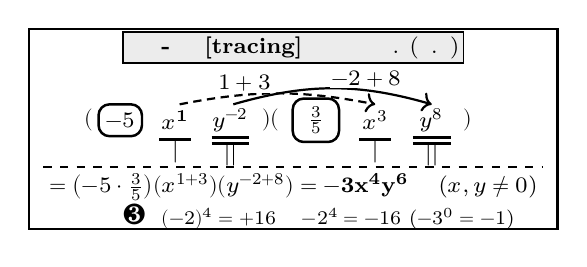
\begin{tikzpicture}[scale=0.92, every node/.style={font=\footnotesize, text=black}]
  \draw[black, line width=0.95pt] (0,0) rectangle (7.30,2.76);
  \node[fill=gray!15, draw=black, line width=0.6pt, inner sep=1.6pt] at (3.65,2.50) {\textbf{កូដ ស-ខ្មៅ \en{[tracing]}៖} លំហាត់គំរូ គ. (ទំ.១៥)};

  % Expression shifted up to leave roomy bottom section for \tfrac{3}{5} and caution
  \node at (0.82,1.50) {$($};
  \node at (1.26,1.50) {$-5$};
  \node at (2.02,1.50) {$x^{\mathbf{1}}$};
  \node at (2.78,1.50) {$y^{-2}$};
  \node at (3.34,1.50) {$)($};
  \node at (3.96,1.50) {$\tfrac{3}{5}$};
  \node at (4.78,1.50) {$x^{3}$};
  \node at (5.56,1.50) {$y^{8}$};
  \node at (6.06,1.50) {$)$};

  % Monochrome B&W circling on coefficients
  \draw[black, line width=0.9pt, rounded corners=4pt] (0.96,1.28) rectangle (1.56,1.72);
  \draw[black, line width=0.9pt, rounded corners=4pt] (3.64,1.20) rectangle (4.28,1.80);

  % Single bar | under x & double bar || under y
  \draw[black, line width=1.05pt] (1.80,1.24) -- (2.24,1.24);
  \draw[black, line width=1.05pt] (4.56,1.24) -- (5.00,1.24);
  \node at (2.02,1.06) {\en{|}};
  \node at (4.78,1.06) {\en{|}};

  \draw[black, line width=1.05pt] (2.52,1.26) -- (3.04,1.26);
  \draw[black, line width=1.05pt] (2.52,1.18) -- (3.04,1.18);
  \draw[black, line width=1.05pt] (5.30,1.26) -- (5.82,1.26);
  \draw[black, line width=1.05pt] (5.30,1.18) -- (5.82,1.18);
  \node at (2.78,1.02) {\en{||}};
  \node at (5.56,1.02) {\en{||}};

  % Overhead exponent arcs (compact, staggered left/right so 0 collision with title or each other)
  \draw[black, densely dashed, line width=0.8pt, ->] (2.08,1.72) to[bend left=11] node[pos=0.32, above=0.3pt, fill=white, inner sep=0.5pt] {$1+3$} (4.78,1.72);
  \draw[black, line width=0.8pt, ->] (2.82,1.72) to[bend left=16] node[pos=0.68, above=0.3pt, fill=white, inner sep=0.5pt] {$-2+8$} (5.56,1.72);

  \draw[black, line width=0.7pt, dashed] (0.20,0.86) -- (7.10,0.86);
  \node at (3.65,0.58) {$= \bigl(-5\cdot\tfrac{3}{5}\bigr)(x^{1+3})(y^{-2+8}) = \mathbf{-3x^4 y^6}$ \quad ($x,y\neq 0$)};
  \node[font=\scriptsize] at (3.65,0.17) {ប្រយ័ត្ន \cnum{3}៖ $(-2)^4=+16$ តែ $-2^4=-16$ ($-3^0=-1$)};
\end{tikzpicture}}

% ៨. E5 Evaluate: កែ Erratum #1 (ប្រតិបត្តិ គ.) និងបិទបេសកកម្ម E1 (2 wide stacked panels)
\newcommand{\figEvaluateRelayErratumEXP}{%
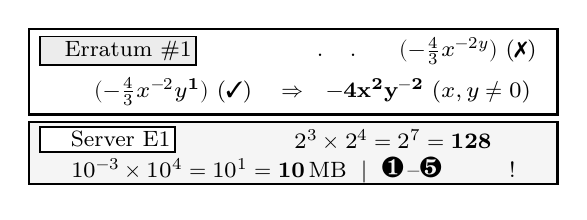
\begin{tikzpicture}[scale=0.92, every node/.style={font=\footnotesize, text=black}]
  % លើ៖ Erratum #1 ក្នុងប្រតិបត្តិ គ.
  \draw[black, line width=0.95pt] (0,0.96) rectangle (7.30,2.14);
  \node[anchor=west, fill=gray!15, draw=black, line width=0.6pt, inner sep=1.6pt] at (0.14,1.84) {កែ \en{Erratum \#1}};
  \node[anchor=east] at (7.14,1.84) {ទំ.១៥ គ. ខុស៖ $(-\tfrac{4}{3}x^{-2y})$ (\ding{55})};
  \node at (3.65,1.28) {កែជា៖ $(-\tfrac{4}{3}x^{-2}y^{\mathbf{1}})$ (\ding{51}) \quad$\Rightarrow$\quad $\mathbf{-4x^2y^{-2}}$ ($x,y\neq 0$)};

  % ក្រោម៖ បិទបេសកកម្ម Server E1
  \draw[black, line width=0.95pt, fill=gray!8] (0,0) rectangle (7.30,0.86);
  \node[anchor=west, fill=white, draw=black, line width=0.6pt, inner sep=1.6pt] at (0.14,0.62) {បិទ \en{Server E1}};
  \node[anchor=east] at (7.14,0.62) {$2^3\times 2^4 = 2^7 = \mathbf{128}$ វីដេអូ};
  \node at (3.65,0.20) {$10^{-3}\times 10^4 = 10^1 = \mathbf{10\unit{MB}}$ \;\textbar{}\; \cnum{1}--\cnum{5}៖ រក្សាគោល!};
\end{tikzpicture}}

% ៩. E5 Diagnostic Exit Foils A–D (4 wide 2-line cards — zero collision!)
\newcommand{\figExitCardsEXPMUL}{%
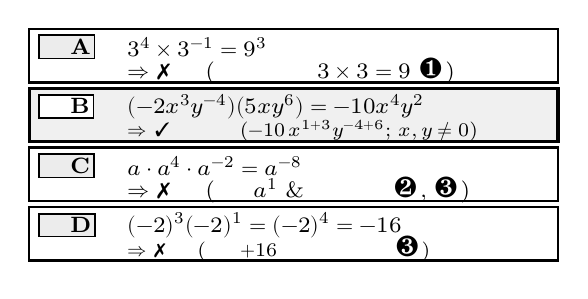
\begin{tikzpicture}[scale=0.92, every node/.style={font=\footnotesize, text=black}]
  % A (X)
  \draw[black, line width=0.85pt] (0,2.46) rectangle (7.30,3.20);
  \node[anchor=west, fill=gray!15, draw=black, line width=0.6pt, inner sep=1.4pt] at (0.12,2.95) {\textbf{កាត \en{A}}};
  \node[anchor=west] at (1.22,2.95) {$3^4\times 3^{-1} = 9^3$};
  \node[anchor=west] at (1.22,2.62) {$\Rightarrow$ \textbf{\ding{55} ខុស} (អន្ទាក់៖ គុណគោល $3\times 3=9$ \cnum{1})};

  % B (CHECK)
  \draw[black, line width=1.15pt, fill=gray!12] (0,1.64) rectangle (7.30,2.38);
  \node[anchor=west, fill=white, draw=black, line width=0.6pt, inner sep=1.4pt] at (0.12,2.13) {\textbf{កាត \en{B}}};
  \node[anchor=west] at (1.22,2.13) {$(-2x^3y^{-4})(5xy^6) = -10x^4y^2$};
  \node[anchor=west, font=\scriptsize] at (1.22,1.80) {\textbf{$\Rightarrow$ \ding{51} ត្រឹមត្រូវ} ($-10\,x^{1+3}y^{-4+6}$; $x,y\neq 0$)};

  % C (X)
  \draw[black, line width=0.85pt] (0,0.82) rectangle (7.30,1.56);
  \node[anchor=west, fill=gray!15, draw=black, line width=0.6pt, inner sep=1.4pt] at (0.12,1.31) {\textbf{កាត \en{C}}};
  \node[anchor=west] at (1.22,1.31) {$a\cdot a^4\cdot a^{-2} = a^{-8}$};
  \node[anchor=west] at (1.22,0.98) {$\Rightarrow$ \textbf{\ding{55} ខុស} (ភ្លេច $a^1$ \& គុណនិទស្សន្ត \cnum{2}, \cnum{3})};

  % D (X)
  \draw[black, line width=0.85pt] (0,0) rectangle (7.30,0.74);
  \node[anchor=west, fill=gray!15, draw=black, line width=0.6pt, inner sep=1.4pt] at (0.12,0.49) {\textbf{កាត \en{D}}};
  \node[anchor=west] at (1.22,0.49) {$(-2)^3(-2)^1 = (-2)^4 = -16$};
  \node[anchor=west, font=\scriptsize] at (1.22,0.16) {$\Rightarrow$ \textbf{\ding{55} ខុស} (ត្រូវ $+16$ ព្រោះគោលមានវង់ក្រចក \cnum{3})};
\end{tikzpicture}}

% ១០. ជំហានទី៥ កិច្ចការផ្ទះ & ស្ពានភ្ជាប់មេរៀន ២.៣ (2 wide stacked panels)
\newcommand{\figHWBridgeEXP}{%
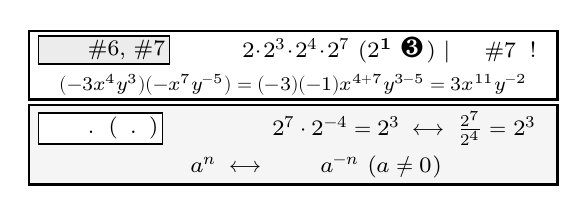
\begin{tikzpicture}[scale=0.92, every node/.style={font=\footnotesize, text=black}]
  % លើ៖ តម្រុយកិច្ចការផ្ទះ #6 ខ & #7 ខ
  \draw[black, line width=0.95pt] (0,1.18) rectangle (7.30,2.12);
  \node[anchor=west, fill=gray!15, draw=black, line width=0.6pt, inner sep=1.6pt] at (0.12,1.86) {តម្រុយ \en{\#6, \#7}};
  \node[anchor=east] at (7.14,1.86) {$2\!\cdot\!2^3\!\cdot\!2^4\!\cdot\!2^7$ ($2^{\mathbf{1}}$ \cnum{3}) \textbar{} ហាម \en{\#7} ក!};
  \node[font=\scriptsize] at (3.65,1.38) {$(-3x^4y^3)(-x^7y^{-5}) = (-3)(-1)x^{4+7}y^{3-5} = 3x^{11}y^{-2}$};

  % ក្រោម៖ ស្ពានភ្ជាប់មេរៀន ២.៣ (ទំ.១៦)
  \draw[black, line width=0.95pt, fill=gray!8] (0,0) rectangle (7.30,1.10);
  \node[anchor=west, fill=white, draw=black, line width=0.6pt, inner sep=1.6pt] at (0.12,0.78) {ស្ពាន ២.៣ (ទំ.១៦)};
  \node[anchor=east] at (7.14,0.78) {$2^7\cdot 2^{-4} = 2^3 \;\longleftrightarrow\; \tfrac{2^7}{2^4} = 2^3$};
  \node at (3.65,0.24) {ចែកនឹង $a^n \;\longleftrightarrow\;$ គុណនឹង $a^{-n}$ ($a\neq 0$)};
\end{tikzpicture}}

% ============================================================================
% ចាប់ផ្ដើមឯកសារ (Document Body — ចំនួនទំព័រ 4–8+ តាមខ្លឹមសារជាក់ស្ដែង, ពេញទំព័រ >=90%)
% ============================================================================
\begin{document}
\fontsize{10pt}{15.2pt}\selectfont

% -------------------- ក្បាលកិច្ចតែងការ (Header) --------------------
\begin{center}
  {\muol\fontsize{11pt}{16pt}\selectfont ព្រះរាជាណាចក្រកម្ពុជា}\\[2pt]
  {\muol\fontsize{10pt}{15pt}\selectfont ជាតិ សាសនា ព្រះមហាក្សត្រ}\\[1pt]
  \khmflourish
\end{center}

\vspace{-28pt}
{\muol\fontsize{9.5pt}{12.5pt}\selectfont
មន្ទីរអប់រំ យុវជន និងកីឡា ខេត្តកំពង់ធំ\\
ការិយាល័យអប់រំ យុវជន និងកីឡា ស្រុកកំពង់ស្វាយ\\
អនុវិទ្យាល័យព្រះក្រសាំង}

\vspace{0pt}
\begin{center}
  {\muol\fontsize{10pt}{14pt}\selectfont កិច្ចតែងការបង្រៀន}
\end{center}
\vspace{-2pt}

% -------------------- ព័ត៌មានទូទៅ (Metadata) --------------------
{\renewcommand{\arraystretch}{0.96}
\hspace*{3.4cm}%
\begin{tabular}{@{}l l L{10.8cm}@{}}
  - \hspace{0.35cm} មុខវិជ្ជា & : & គណិតវិទ្យា ថ្នាក់ទី៨ \\
  - \hspace{0.35cm} ចំណងជើងមេរៀន & : & មេរៀនទី២ ស្វ័យគុណ \\
  - \hspace{0.35cm} ចំណងជើងរង & : & ២.២. វិធីគុណស្វ័យគុណមាននិទស្សន្តរ៉ឺឡាទីប (ទំ.១៥ និង ២៥) \\
  - \hspace{0.35cm} រយៈពេល & : & ១ ម៉ោងសិក្សា (៥០ នាទី) \\
  - \hspace{0.35cm} បង្រៀនដោយ & : & ហុក ប៊ុនថែន \\
  - \hspace{0.35cm} កាលបរិច្ឆេទ & : & ថ្ងៃចន្ទ ទី១៦ ខែវិច្ឆិកា ឆ្នាំ២០២៦ \\
\end{tabular}

\vspace{1pt}

% -------------------- I. វត្ថុបំណង --------------------
\textbf{I.} {\muol វត្ថុបំណង}\\[1pt]
\hspace*{0.55cm}%
\begin{tabular}{@{}l l L{14.2cm}@{}}
  \wcirc \hspace{0.25cm} វិជ្ជាសម្បទា & : & សិស្សបង្គុំនិងប្រាប់វិធានគុណស្វ័យគុណគោលដូចគ្នា $a^m \cdot a^n = a^{m+n}$ ($a$ ជាចំនួនសនិទាន, $m, n \in \mathbb{Z}$, និងលក្ខខណ្ឌ $a \neq 0$ កាលណា $m \le 0$ ឬ $n \le 0$) ព្រមទាំងភ្ជាប់ស្ពាន $a^0 = 1$ និង $a^{-n} = \frac{1}{a^n}$ បានត្រឹមត្រូវ ។ \\
  \wcirc \hspace{0.25cm} បំណិនសម្បទា & : & សិស្សអនុវត្តបន្ទះកត្តា \en{1:1} ($2^3\times 2^4$), ផ្ទាំងបន្សាបគូសូន្យ \en{1:1} ($10^{-3}\times 10^4$), \en{Dual POE 2A--2B}, កូដ ស-ខ្មៅ \textbf{[tracing]} (ព័ទ្ធមេគុណ, គូស \en{|}, \en{||}, ធ្នូនិទស្សន្ត) និងធនាគារ \cnum{1}--\cnum{5} ដោះស្រាយលំហាត់គំរូ ប្រតិបត្តិ (ទំ.១៥ កែ \en{Erratum \#1}) និងលំហាត់ \en{\#6--\text{\#7}} (ទំ.២៥) បានត្រឹមត្រូវ ។ \\
  \wcirc \hspace{0.25cm} ចរិយាសម្បទា & : & សហការក្នុងក្រុម ៣ នាក់ («ក្រុមវិស្វករទិន្នន័យ និងគូសូន្យ ៣ តួនាទី») តាមវិន័យ \en{Pause-Ask! / Pause-Review!} និងប្រុងប្រយ័ត្នចំពោះអន្ទាក់គុណគោល គុណនិទស្សន្ត និទស្សន្តលាក់ \en{1} និងសញ្ញាដកមុខវង់ក្រចក ។ \\
\end{tabular}

\vspace{1pt}

% -------------------- II. សម្ភារៈឧបទេស --------------------
\textbf{II.} {\muol សម្ភារៈឧបទេស}\\[1pt]
\hspace*{0.55cm}$\bullet$ \hspace{0.35cm} សៀវភៅគោលថ្នាក់ទី៨ (ទំ.១៤--១៦, ២៥) បន្ទាត់ក្រិត \en{1:1} កន្ត្រៃ ខ្មៅដៃគូស \textbf{[tracing]} សម្ភារៈ \en{1:1} (\en{P1} ទំព័រ ១) កាតស៊ើបអង្កេត \en{E4} (\en{P2} ទំព័រ ២) សន្លឹក \en{Relay} ៣ តួនាទី (\en{P3} ទំព័រ ៣) ផ្ទាំងធនាគារ \cnum{1}--\cnum{5} (\en{P4} ទំព័រ ៤) កាត \en{A--D} \en{\& Exit Ticket} (\en{P5} ទំព័រ ៥) និងប័ណ្ណកិច្ចការផ្ទះ (\en{P6} ទំព័រ ៦) ។

\vspace{1pt}

% -------------------- III. វិធីសាស្រ្តបង្រៀន --------------------
\textbf{III.} {\muol វិធីសាស្រ្តបង្រៀន}\\[1pt]
\hspace*{0.45cm}%
\begin{tabular}{@{}l l L{14.85cm}@{}}
  $\bullet$ \hspace{0.25cm} គោលវិធី & : & សិស្សមជ្ឈមណ្ឌល \\
  $\bullet$ \hspace{0.25cm} យុទ្ធវិធីបង្រៀន & : & ស្ថាបនានិយម គំរូ \en{5Es} (បន្ទះកត្តា \en{1:1}, បន្សាបគូសូន្យ, \en{Dual POE 2A--2B}, \textbf{[tracing]}, ធនាគារ \cnum{1}--\cnum{5}, \en{Relay} ៣ តួនាទី) \\
\end{tabular}
}

\vspace{1pt}

% -------------------- IV. ដំណើរការបង្រៀន --------------------
\textbf{IV.} {\muol ដំណើរការបង្រៀន}

\vspace{1pt}

% ============================================================================
% តារាងដំណើរការបង្រៀន (Granular 2-5 Line Sub-Rows, Dedicated TikZ Rows, 50 min)
% ============================================================================
\renewcommand{\arraystretch}{1.15}
\begin{longtable}{|L{5.50cm}|L{7.90cm}|L{4.80cm}|}
\hline
\rowcolor{headgray}
\multicolumn{1}{|c|}{\muol សកម្មភាពគ្រូ} &
\multicolumn{1}{c|}{\muol ខ្លឹមសារមេរៀន} &
\multicolumn{1}{c|}{\muol សកម្មភាពសិស្ស} \\
\hline
\endfirsthead

\hline
\endhead

\hline
\endfoot

\hline
\endlastfoot

% ==================== ជំហានទី១ (2min) ====================
\stepheader{ជំហានទី១ \enbf{(}រដ្ឋបាលថ្នាក់\enbf{)}}
$\bullet$ ពិនិត្យអវត្តមាន អនាម័យ និងសណ្ដាប់ធ្នាប់ថ្នាក់រៀន
&
$\bullet$ រដ្ឋបាលថ្នាក់\par\vspace{2pt}
$\bullet$ អនាម័យ និងសុវត្ថិភាពកន្ត្រៃ/បន្ទាត់
&
$\circ$ ប្រធានថ្នាក់រាយការណ៍អវត្តមាន \\[3pt]

$\bullet$ រៀបចំសិស្សជាក្រុម ៣ នាក់ («ក្រុមវិស្វករទិន្នន័យ និងគូសូន្យ ៣ តួនាទី»)\par\vspace{2pt}
$\bullet$ ចែកសម្ភារៈ \en{P1} (ទំព័រ ១) ផ្កាប់លើតុ
&
$\bullet$ ត្រៀមក្រុម ៣ នាក់ និងរៀបចំសម្ភារៈ \en{B\&W} (កន្ត្រៃ បន្ទាត់ \en{1:1} ខ្មៅដៃ)
&
$\circ$ អង្គុយតាមក្រុម ៣ នាក់ និងដាក់ \en{P1} ផ្កាប់លើតុ \\
\hline

% ==================== ជំហានទី២ (9min: <=3 + 3 + E1 3) ====================
\stepheader{ជំហានទី២ \enbf{(}កិច្ចការផ្ទះ \enbf{+} ទំនាក់ទំនងមេរៀនថ្មី\enbf{)}}
% --- ២.១ កំណែកិច្ចការផ្ទះ (<=3min) ---
\ditem \textbf{កំណែកិច្ចការផ្ទះ ($\le 3\unit{min}$)} \timenote{(កុំសរសេរវែង)}\par\vspace{2pt}
$\bullet$ ហៅសិស្សផ្ទៀង \textbf{២.១ ប្រតិបត្តិ 2 គ.} (ទំ.១៤) និង \textbf{\#1 ខ.} (ទំ.២៥)\par\vspace{2pt}
\hspace*{0.3em}– \textbf{សំណួរ៖} «ហេតុអ្វីត្រូវរក្សាវង់ក្រចក $(-8)^6$ ជំនួស $-8^6$?»
&
{\centering\redsub{កំណែកិច្ចការផ្ទះមេរៀនមុន (២.១)}\par}\par\vspace{2pt}
$\bullet$ \textbf{ប្រតិបត្តិ 2 គ. (ទំ.១៤)៖} $(-2)^7 = -128$ (៧ កត្តាសេស)\par\vspace{2pt}
$\bullet$ \textbf{\#1 ខ.} $\underbrace{(-8)\cdots(-8)}_{6\text{ កត្តា}} = (-8)^6$ \mbox{(គោល $-8$)}
&
$\circ$ ផ្ទៀងចម្លើយក្នុងសៀវភៅ\par\vspace{2pt}
$\circ$ ឆ្លើយ៖ «គោលអវិជ្ជមានត្រូវមានវង់ក្រចក!» \\[3pt]

% --- ២.២ រំលឹកមេរៀនទាក់ទង (3min) ---
\ditem \textbf{រំលឹកមេរៀនទាក់ទង (3min)}\par\vspace{2pt}
$\bullet$ រំលឹក $a^n$, និទស្សន្តលាក់ \en{1} និងបូកចំនួនគត់រ៉ឺឡាទីប\par\vspace{2pt}
\hspace*{0.3em}– \textbf{សំណួរ៖} «គណនា $-3+4$, $-2+8$, $-3+1$»
&
{\centering\redsub{រំលឹកមេរៀនទាក់ទងមេរៀនថ្មី}\par}\par\vspace{2pt}
$\bullet$ $a^n = \underbrace{a\cdot a\cdots a}_{n\text{ កត្តា}}$ និងនិទស្សន្តលាក់ $x = x^1,\; 2 = 2^1$\par\vspace{2pt}
$\bullet$ បូកចំនួនគត់៖ $-3+4 = 1$,\quad $-2+8 = 6$,\quad $-3+1 = -2$
&
$\circ$ ឆ្លើយរហ័ស៖ «$1$, $6$, $-2$» និង $x=x^1$ \\[3pt]

$\bullet$ ដឹកនាំលំនាំចែកគោល ១០ បង្កើតស្ពាន $a^0$ និង $a^{-n}$ ($a\neq 0$)\par\vspace{2pt}
\hspace*{0.3em}– \textbf{សំណួរ៖} «ពី $10^2 \to 10^1$ ចែកនឹង ១០ តើ $10^0$ និង $10^{-1}, 10^{-3}$ ស្មើប៉ុន្មាន?»
&
$\bullet$ \textbf{លំនាំចែកគោល ១០ ($a\neq 0$)៖}\par\vspace{2pt}
$10^2=100 \xrightarrow{\div 10} 10^1=10 \xrightarrow{\div 10} \mathbf{10^0=1}$\par\vspace{2pt}
$\xrightarrow{\div 10} 10^{-1}=\dfrac{1}{10} \longrightarrow 10^{-3}=\dfrac{1}{10^3}$
&
$\circ$ រកឃើញ៖ $10^0=1$ និង $10^{-3}=\frac{1}{10^3}$ \\[3pt]

&
\cfig{\figStepTwoReviewEXP}
& \\[3pt]

% --- ២.៣ E1 Engage (3min) ---
\fiveE{E1 - Engage (3min)} \timenote{(កុំទាន់ផ្ដល់ចម្លើយ)}\par\vspace{2pt}
\ditem \textbf{បេសកកម្មឃ្លាំងវីដេអូ \en{Server} បណ្ណាល័យឌីជីថលអនុវិទ្យាល័យព្រះក្រសាំង}\par\vspace{2pt}
$\bullet$ បង្ហាញស្ថានភាព \en{Server} ថតវីដេអូ និងកញ្ចប់បង្ហាប់
&
{\centering\redsub{បេសកកម្ម \en{E1}៖ ឃ្លាំងវីដេអូ \en{Server} បណ្ណាល័យឌីជីថល}\par}\par\vspace{2pt}
$\bullet$ \textbf{ក. ចំនួនវីដេអូ៖} មាន $2^3$ ថត ហើយ ១ ថតមាន $2^4$ វីដេអូ $\to 2^3 \times 2^4 = ?$\par\vspace{2pt}
$\bullet$ \textbf{ខ. ទំហំបង្ហាប់៖} កញ្ចប់ $10^{-3}\unit{MB} \times 10^4$ ឯកសារ $\to 10^{-3}\times 10^4 = ?$
&
$\circ$ សង្កេតស្ថានភាព \en{Server} បណ្ណាល័យឌីជីថល \\[3pt]

&
\cfig{\figEngageServerEXP}
& \\[3pt]

\hspace*{0.3em}– \textbf{សំណួរទស្សន៍ទាយ \en{(POE)}៖} «តើ $2^3\times 2^4$ ស្មើ $2^7$, $4^7$ ឬ $2^{12}$? ហើយ $10^{-3}\times 10^4$ យកនិទស្សន្ត $(-3)+4$ ឬ $(-3)\times 4$?»
&
\textbf{ការទស្សន៍ទាយក្រុម (កត់ទុកលើក្ដារខៀន)៖}\par\vspace{2pt}
១) $2^3\times 2^4$៖ $2^7$ \textbar{} $4^7$ \textbar{} $2^{12}$?\par\vspace{2pt}
២) $10^{-3}\times 10^4$៖ $(-3)+4$ ឬ $(-3)\times 4$?
&
$\circ$ ពិភាក្សាក្រុម និងបោះឆ្នោតទស្សន៍ទាយ (រង់ចាំផ្ទៀងនៅ \fiveE{E5}) \\
\hline

% ==================== ជំហានទី៣ (17min: E2 11m + E3 6m) ====================
\stepheader{ជំហានទី៣ \enbf{(}ខ្លឹមសារមេរៀនថ្មី\enbf{)}}
% --- ៣.១ ចំណងជើង & E2 Act 1 (6min) ---
\fiveE{E2 - Explore (11min)}\par\vspace{2pt}
$\bullet$ សរសេរចំណងជើងមេរៀនលើក្ដារខៀន
&
មេរៀនទី២ \hspace{0.1cm} {\muol ស្វ័យគុណ} \textbf{(ត)}\par\vspace{2pt}
\textbf{២.២. វិធីគុណស្វ័យគុណមាននិទស្សន្តរ៉ឺឡាទីប}
&
$\circ$ កត់ចំណងជើងមេរៀនចូលសៀវភៅ \\[3pt]

\ditem \textbf{សកម្មភាព ១៖ ពិសោធន៍ \en{P1 1:1} (6min)}\par\vspace{2pt}
$\bullet$ ផ្ទៀងបន្ទះក្រិត $5.00\unit{cm}$ (\en{Actual Size 100\%})\par\vspace{2pt}
$\bullet$ \textbf{១ក៖} កាត់បន្ទះ $2^3$ ($3.00\unit{cm}$) និង $2^4$ ($4.00\unit{cm}$) ដាក់តគ្នាលើផ្លូវ $0\text{--}8\unit{cm}$
&
\textbf{១ក. បន្ទះកត្តា \en{1:1} ($2^3 \times 2^4$)៖}\par\vspace{2pt}
$3.00\unit{cm} + 4.00\unit{cm} = 7.00\unit{cm}$ ($7$ កត្តានៃ $2$)\par\vspace{2pt}
$\Rightarrow 2^3 \times 2^4 = 2^{3+4} = \mathbf{2^7}$ (រក្សាគោល $2$ ដដែល!)
&
$\circ$ ផ្ទៀងក្រិត $5.00\unit{cm}$, កាត់ និងតភ្ជាប់បន្ទះ $3+4=7\unit{cm}$ \\[3pt]

&
\cfig{\figExploreStripsEXP}
& \\[3pt]

$\bullet$ \textbf{១ខ៖} ផ្ទៀងផ្ទាំងបន្សាបគូសូន្យ \en{1:1} ($10^{-3}\times 10^4$)\par\vspace{2pt}
\hspace*{0.3em}– \textbf{សំណួរ៖} «ពេលគូសឆ្នូត \en{/} កាត់គូ $\frac{1}{10}\times 10=1$ អស់ ៣ គូ តើនៅសល់ប្រវែងប៉ុន្មាន?»
&
\textbf{១ខ. ផ្ទាំងបន្សាបគូសូន្យ \en{1:1} ($10^{-3}\times 10^4$)៖}\par\vspace{2pt}
បន្សាប ៣ គូ ($\frac{1}{10}\cdot 10 = 10^0 = 1$) $\Rightarrow$ សល់ $1.00\unit{cm}$\par\vspace{2pt}
$\Rightarrow 10^{-3}\times 10^4 = 10^{-3+4} = \mathbf{10^1 = 10\unit{MB}}$
&
$\circ$ គូសឆ្នូត \en{/} កាត់ ៣ គូ និងអានលទ្ធផល $10^1 = 10\unit{MB}$ \\[3pt]

&
\cfig{\figExploreZeroPairEXP}
& \\[3pt]

% --- ៣.២ E2 Act 2 Dual POE (5min) ---
\ditem \textbf{សកម្មភាព ២៖ \en{Dual POE 2A--2B} (5min, \en{P1})}\par\vspace{2pt}
$\bullet$ \textbf{\en{POE 2A} (អន្ទាក់គុណគោល)៖} ឱ្យសិស្សទស្សន៍ទាយមុន ទើបគណនាតម្លៃលេខពិត $2^3\cdot 2^4 \stackrel{?}{=} 4^7$ និង $2^3\cdot 3^2 \stackrel{?}{=} 6^5$
&
\textbf{\en{POE 2A}៖ ទាត់ចោលការគុណគោល៖}\par\vspace{2pt}
$\bullet$ $2^3\cdot 2^4 = 8\times 16 = 128 = 2^7 \neq 4^7 = 16,384$\par\vspace{2pt}
$\bullet$ $2^3\cdot 3^2 = 8\times 9 = 72 \neq 6^5 = 7,776$ (គោលខុសគ្នា!)
&
$\circ$ ទស្សន៍ទាយ គណនាផ្ទៀង និងបដិសេធ $4^7, 6^5$ \\[3pt]

&
\cfig{\figExplorePOETwoAEXP}
& \\[3pt]

$\bullet$ \textbf{\en{POE 2B} (អន្ទាក់គុណនិទស្សន្ត និងលាក់ \en{1})៖} ពិនិត្យរូបប្លុក/ក្រឡាបង្វិល $25^\circ$៖ $3^2\cdot 3^3 \stackrel{?}{=} 3^6$ និង $a\cdot a^3 \stackrel{?}{=} a^3$\par\vspace{2pt}
\hspace*{0.3em}– \textbf{សំណួរ៖} «សាកល្បង $a=2$ តើ $2\cdot 2^3$ ស្មើ $2^3$ ឬ $2^4$?»
&
\textbf{\en{POE 2B}៖ ទាត់ចោលការគុណនិទស្សន្ត \& ភ្លេច \en{1}៖}\par\vspace{2pt}
$\bullet$ $3^2\cdot 3^3 = 9\times 27 = 243 = 3^5 \neq 3^6 = 729$\par\vspace{2pt}
$\bullet$ $a\cdot a^3 = a^{\mathbf{1}}\cdot a^3 = a^{1+3} = a^4 \neq a^3$ (មាន ៤ កត្តា!)
&
$\circ$ ផ្ទៀង $3^5\neq 3^6$ និងបញ្ជាក់ $a=a^{\mathbf{1}}$ \\[3pt]

&
\cfig{\figExplorePOETwoBEXP}
& \\[3pt]

% --- ៣.៣ E3 Explain (6min) ---
\fiveE{E3 - Explain (6min)}\par\vspace{2pt}
\ditem \textbf{សិស្សបង្គុំឧទាហរណ៍ និងទ្រឹស្ដីបទ (ទំ.១៥)}\par\vspace{2pt}
$\bullet$ ឱ្យសិស្សសង្ខេបលំនាំ \textbf{ឧទាហរណ៍ ក--ឃ} មុនគ្រូ\par\vspace{2pt}
\hspace*{0.3em}– \textbf{សំណួរ៖} «បើ $a=0$ និង $m=-2$ តើ $0^{-2}$ មានន័យទេ?»
&
\textbf{ឧទាហរណ៍ (ទំ.១៥)៖}\par\vspace{2pt}
$\bullet$ \textbf{ក.} $2^3\times 2^4 = 2^{3+4} = 2^7$ \quad \textbar{} \quad \textbf{ខ.} $3^5\times 3^7 = 3^{5+7} = 3^{12}$\par\vspace{2pt}
$\bullet$ \textbf{គ.} $\left(\frac{3}{2}\right)^2\cdot\left(\frac{3}{2}\right)^3 = \left(\frac{3}{2}\right)^5$ \quad \textbar{} \quad \textbf{ឃ.} $a^m\cdot a^n = a^{m+n}$
&
$\circ$ សិស្សឡើងសង្ខេបលំនាំ $a^m\cdot a^n = a^{m+n}$ និងឆ្លើយ $a\neq 0$ \\[3pt]

$\bullet$ ចាក់សោប្រអប់ \textbf{«ជាទូទៅ»} និងកែ \textbf{\en{Erratum \#2}} ($a\neq 0$ ពេលនិទស្សន្ត $\le 0$, និងស្ពាន $a^0=1, a^{-n}=\frac{1}{a^n}$)
&
\textbf{ជាទូទៅ (ទំ.១៥ កែ \en{Erratum \#2})៖}\par\vspace{2pt}
បើ $a$ ជាចំនួនសនិទាន (\graybox{\textbf{$a \neq 0$ បើ $m \le 0$ ឬ $n \le 0$}}) និង $m,n \in \mathbb{Z}$ នោះ៖ \graybox{$a^m \cdot a^n = a^{m+n}$} ។\par\vspace{2pt}
\timenote{បន្ថែមស្ពាន៖ $a^0=1$ និង $a^{-n}=\frac{1}{a^n}$ ($a\neq 0$)}
&
$\circ$ កត់ប្រអប់ «ជាទូទៅ» និងបន្ថែមលក្ខខណ្ឌ $a\neq 0$ ក្នុងសៀវភៅ \\[3pt]

$\bullet$ សង្ខេបជាតារាង \textbf{សម្មតិកម្ម--សន្និដ្ឋាន--វិបាក}
&
{\fontsize{8.8pt}{12.6pt}\selectfont\setlength{\tabcolsep}{2.4pt}\renewcommand{\arraystretch}{1.12}%
\centering
\begin{tabular}{|L{2.25cm}|L{2.35cm}|L{2.65cm}|}
  \hline
  \cellcolor{headgray}\textbf{សម្មតិកម្ម} & \cellcolor{headgray}\textbf{សន្និដ្ឋាន} & \cellcolor{headgray}\textbf{វិបាក / អន្ទាក់} \\
  \hline
  គោលដូចគ្នា $a^m\cdot a^n$ ($a\neq 0$ បើ $\le 0$) & $a^m\cdot a^n = a^{m+n}$ (រក្សាគោល បូកនិទស្សន្ត) & $2^3\cdot 2^4 = 2^7 \neq 4^7$;\par $2^3\cdot 3^2 \neq 6^5$;\par $3^2\cdot 3^3 = 3^5 \neq 3^6$ \\[2pt]
  \hline
\end{tabular}\par}
&
$\circ$ ផ្ទៀងតារាង សម្មតិកម្ម--សន្និដ្ឋាន--វិបាក \\[3pt]

\cnum{1}--\cnum{3} បិទផ្ទាំង \textbf{ធនាគារហេតុផល \cnum{1}--\cnum{5}} (\en{P4} ទំព័រ ៤) និងផ្ទៀង \cnum{1}--\cnum{3}
&
\textbf{ធនាគារហេតុផល \cnum{1}--\cnum{3} (\en{P4})៖}\par\vspace{2pt}
\cnum{1} ច្រកគោលដូចគ្នា (\en{Same-Base})៖ ហាមគុណគោល\par\vspace{2pt}
\cnum{2} វិធាន $a^m\cdot a^n = a^{m+n}$ ($a\neq 0$ បើ $\le 0$)\par\vspace{2pt}
\cnum{3} និទស្សន្តលាក់ \en{1} ($x^1, y^1, 2^1$) \& ដែនវង់ក្រចក
&
$\circ$ អាន និងផ្ទៀង \cnum{1}--\cnum{3} លើផ្ទាំងទំព័រ ៤ \\[3pt]

\cnum{4}--\cnum{5} ផ្ទៀងកូដផ្ដុំមេគុណ--អញ្ញាត និងស្ពាន $a^{-n}, a^0$
&
\textbf{ធនាគារហេតុផល \cnum{4}--\cnum{5} (\en{P4})៖}\par\vspace{2pt}
\cnum{4} ផ្ដុំមេគុណ (ព័ទ្ធរង្វង់) \& គោលដូចគ្នា (\en{|}, \en{||}, ធ្នូ)\par\vspace{2pt}
\cnum{5} ស្ពាន $a^{-n}=\frac{1}{a^n}$, $a^0=1$ ($a\neq 0$) និងបន្សាបគូសូន្យ
&
$\circ$ ផ្ទៀង \cnum{4}--\cnum{5} លើផ្ទាំងទំព័រ ៤ \\
\hline

% ==================== ជំហានទី៤ (20min: E4 10m + E5 10m) ====================
\stepheader{ជំហានទី៤ \enbf{(}ពង្រីកចំណេះដឹង\enbf{)}}
% --- ៤.១ E4 Elaborate (10min) ---
\fiveE{E4 - Elaborate (10min)}\par\vspace{2pt}
\ditem ចែក \textbf{កាតស៊ើបអង្កេត ៣ ជំហាន \en{B\&W}} (\en{P2} ទំព័រ ២)\par\vspace{2pt}
$\bullet$ ដឹកនាំ \textbf{លំហាត់គំរូ ក, ខ} (ទំ.១៥) ភ្ជាប់ \cnum{1}, \cnum{2}, \cnum{4}
&
{\muol លំហាត់គំរូ} \textbf{(ទំ.១៥ — ក, ខ)៖}\par\vspace{2pt}
$\bullet$ \textbf{ក.} $10^{-3}\times 10^4 = 10^{-3+4} = 10^1 = 10$ \quad (\cnum{1}, \cnum{2})\par\vspace{2pt}
$\bullet$ \textbf{ខ.} $(-5y^2)(7y^8) = (-5\cdot 7)(y^2\cdot y^8) = -35y^{10}$ \quad (\cnum{4}, \cnum{2})
&
$\circ$ ទទួលកាត \en{P2} និងដោះស្រាយ \textbf{ក, ខ} \\[3pt]

$\bullet$ បង្ហាញកូដ ស-ខ្មៅ \textbf{[tracing]} លើ \textbf{លំហាត់គំរូ គ.} ($x,y\neq 0$)៖ ព័ទ្ធរង្វង់ \circbox{-5}, \circbox{\tfrac{3}{5}}, គូស \en{|} ក្រោម $x^1, x^3$, គូស \en{||} ក្រោម $y^{-2}, y^8$
&
$\bullet$ \textbf{គ.} $(-5xy^{-2})\left(\dfrac{3}{5}x^3 y^8\right)$ ($x,y\neq 0$)\par\vspace{2pt}
$= -\left(5\times\dfrac{3}{5}\right)(x^{\mathbf{1}}\cdot x^3)(y^{-2}\cdot y^8)$ \quad (\cnum{3}, \cnum{4})\par\vspace{2pt}
$= -3 \cdot x^{1+3} \cdot y^{-2+8} = \graybox{$-3x^4 y^6$}$ \quad (\cnum{2})
&
$\circ$ ព័ទ្ធមេគុណ គូស \en{|}, \en{||}, ធ្នូ \textbf{[tracing]} និងរក $-3x^4y^6$ \\[3pt]

&
\cfig{\figElaborateTracingEXP}
& \\[3pt]

$\bullet$ សួរសំណួរ \textbf{\en{EIA Looking-Back}} (៣០ វិនាទី) ផ្ទៀងសញ្ញាដក និងនិទស្សន្តលាក់ \en{1}
&
\textbf{\en{EIA Looking-Back} (ពិនិត្យត្រឡប់)៖}\par\vspace{2pt}
១) តើសញ្ញាដកមុខ $-5$ រក្សាទុកឬនៅ? ($\to -35, -3$)\par\vspace{2pt}
២) ហេតុអ្វី $x\cdot x^3 = x^4$ ($\neq x^3$) និង $y^{-2}\cdot y^8 = y^6$?
&
$\circ$ ឆ្លើយ៖ «រក្សាសញ្ញាដក, $x=x^1 \Rightarrow 1+3=4$ និង $-2+8=6$» \\[3pt]

% --- ៤.២ E5 Evaluate: 3-Role Relay (5min, P3) ---
\fiveE{E5 - Evaluate (10min)}\par\vspace{2pt}
\ditem \textbf{\en{Relay} ៣ តួនាទី (5min, \en{P3} ទំព័រ ៣)}\par\vspace{2pt}
$\bullet$ \textbf{តួនាទី ១ (\en{Pause-Ask!})}៖ គូស \textbf{[tracing]} និងសួរកែ \en{Erratum \#1}\par\vspace{2pt}
$\bullet$ \textbf{តួនាទី ២}៖ គណនាភ្ជាប់ \cnum{1}--\cnum{5}
&
{\muol លំហាត់ប្រតិបត្តិ} \textbf{(ទំ.១៥ — ក, ខ)៖}\par\vspace{2pt}
$\bullet$ \textbf{ក.} $x^9\cdot x^4 = x^{9+4} = x^{13}$ \quad (\cnum{1}, \cnum{2})\par\vspace{2pt}
$\bullet$ \textbf{ខ.} $\left(-\dfrac{3}{2}\right)^2\cdot\left(-\dfrac{3}{2}\right)^{-2} = \left(-\dfrac{3}{2}\right)^0 = 1$ \quad (\cnum{2}, \cnum{5})
&
$\circ$ អនុវត្តតួនាទី ១--២ និងហៅ \en{Pause-Ask!} \\[3pt]

$\bullet$ \textbf{តួនាទី ៣ (\en{Pause-Review!})}៖ ផ្ទៀងសញ្ញា និងបកស្រាយ \textbf{\en{Erratum \#1}} ក្នុង \textbf{ប្រតិបត្តិ គ.}\par\vspace{2pt}
\timenote{(កែ $x^{-2y} \to x^{-2}y$ ក្នុងសៀវភៅទំ.១៥!)}
&
$\bullet$ \textbf{គ. [កែ \en{Erratum \#1}]៖} $(3x^4y^{-3})\left(-\dfrac{4}{3}x^{-2}y^{\mathbf{1}}\right)$\par\vspace{2pt}
$= \left(3\times\left(-\dfrac{4}{3}\right)\right)(x^{4+(-2)})(y^{-3+1}) = \graybox{$-4x^2 y^{-2}$}$ ($x,y\neq 0$; \cnum{3}, \cnum{4}, \cnum{2})
&
$\circ$ តួនាទី ៣ ផ្ទៀង $-4$, $y^{-2}$, $\left(-\frac{3}{2}\right)^0=+1$ (\en{Pause-Review!}) \\[3pt]

&
\cfig{\figEvaluateRelayErratumEXP}
& \\[3pt]

$\bullet$ \textbf{បិទបេសកកម្ម \en{Server E1}៖} ផ្ទៀងការទស្សន៍ទាយដើមម៉ោងលើក្ដារខៀន
&
\textbf{បិទបេសកកម្ម \en{E1}៖} ១) $2^3\times 2^4 = 2^7 = \mathbf{128}$ វីដេអូ \quad\textbar{}\quad ២) $10^{-3}\times 10^4 = 10^1 = \mathbf{10\unit{MB}}$ ។
&
$\circ$ ផ្ទៀងទស្សន៍ទាយ \en{E1} និងកែតម្រូវការយល់ខុស \\[3pt]

% --- ៤.៣ E5 Evaluate: Exit Foils A-D & 3-Q Exit Ticket (5min, P5) ---
\ditem \textbf{កាត \en{A--D} និងសំបុត្រចេញ (5min, \en{P5} ទំព័រ ៥)}\par\vspace{2pt}
$\bullet$ បង្ហាញកាត \en{A--D} ឱ្យសិស្សលើកមេដៃ \ding{51} ឬខ្វែងដៃ \ding{55} និងម្រាមដៃ \en{1--5}
&
{\centering\textbf{កាតវិនិច្ឆ័យរហ័ស \en{A--D} (\en{P5} ទំព័រ ៥)}\par}
&
$\circ$ សង្កេតកាត \en{A--D} និងលើកសញ្ញាឆ្លើយ \\[3pt]

&
\cfig{\figExitCardsEXPMUL}
& \\[3pt]

$\bullet$ បញ្ជាក់ចម្លើយ \en{A--D} និងចែក \textbf{សំបុត្រចេញ ៣ សំណួរ} (៦០--៩០ វិនាទី)
&
$\bullet$ \textbf{ចម្លើយ \en{A--D}៖} \en{A} (\ding{55} \cnum{1}) \textbar{} \graybox{\textbf{\en{B} (\ding{51})}} \textbar{} \en{C} (\ding{55} $a^3$) \textbar{} \en{D} (\ding{55} $+16$)\par\vspace{2pt}
$\bullet$ \textbf{សំបុត្រចេញ៖} ១) $5^{-2}\cdot 5^6 = 5^4$ ($625$); ២) $(-4x)(2x^{-3}y^2) = -8x^{-2}y^2$ ($x\neq 0$); ៣) $2^3\cdot 3^2 \neq 6^5$ (គោលខុសគ្នា \cnum{1})
&
$\circ$ បំពេញ និងប្រគល់សំបុត្រចេញ ៣ សំណួរ \\
\hline

% ==================== ជំហានទី៥ (<=2min) ====================
\stepheader{ជំហានទី៥ \enbf{(}កិច្ចការផ្ទះ \enbf{+} បណ្ដាំផ្ញើ\enbf{)}}
\timenote{ចំណាយពេលឱ្យតិចបំផុតកុំឱ្យលើស 2min}\par\vspace{2pt}
$\bullet$ ចែកប័ណ្ណកិច្ចការផ្ទះ (\en{P6} ទំព័រ ៦)\par\vspace{2pt}
$\bullet$ ណែនាំ \textbf{ផ្នែក ក} (ទំ.២៥ \en{\#6} ក, ខ, គ)
&
{\centering{\muol កិច្ចការផ្ទះ} \textbf{(សៀវភៅគោល ទំ.២៥)}\par}\par\vspace{2pt}
\textbf{ផ្នែក ក (លំហាត់ \en{\#6} ក, ខ, គ)៖}\par\vspace{2pt}
$\bullet$ \textbf{ក.} $(4^5)(4^2)(4^4) = 4^{11}$\par\vspace{2pt}
$\bullet$ \textbf{ខ.} $2\times 2^3\times 2^4\times 2^7 = 2^{1+3+4+7} = 2^{15}$ ($2=2^1$)\par\vspace{2pt}
$\bullet$ \textbf{គ.} $\left(\frac{4}{3}\right)^4\left(\frac{4}{3}\right)^{-6}\left(\frac{4}{3}\right)^3 = \left(\frac{4}{3}\right)^1 = \frac{4}{3}$
&
$\circ$ ទទួលប័ណ្ណកិច្ចការផ្ទះ និងកត់ត្រាផ្នែក ក \\[3pt]

$\bullet$ ណែនាំ \textbf{ផ្នែក ខ} (ទំ.២៥ \en{\#7} ខ និងស្ពានមេរៀន ២.៣)\par\vspace{2pt}
\timenote{(បញ្ជាក់ជៀសវាង \en{\#7} ក ដែលបោះពុម្ពខ្វះតួ និង \en{\#6} ឃ)}
&
\textbf{ផ្នែក ខ (លំហាត់ \en{\#7} ខ និងស្ពាន ២.៣)៖}\par\vspace{2pt}
$\bullet$ \textbf{\#7 ខ.} $(-3x^4y^3)(-x^7y^{-5}) = 3x^{11}y^{-2}$ ($y\neq 0$; $-x^7=(-1)x^7$)\par\vspace{2pt}
$\bullet$ \textbf{ស្ពាន ២.៣៖} គណនានិងប្រៀបធៀប $2^7\cdot 2^{-4}$ និង $\dfrac{2^7}{2^4}$
&
$\circ$ កត់ត្រាផ្នែក ខ និងគូសចំណាំជៀសវាង \en{\#7} ក \\[3pt]

&
\cfig{\figHWBridgeEXP}
& \\[3pt]

$\bullet$ សង្ខេបខ្លឹមសារ ផ្ដាំអានមុន \textbf{៣. វិធីចែកស្វ័យគុណ (ទំ.១៦)} និងអប់រំសីលធម៌
&
$\bullet$ \textbf{សង្ខេប៖} រក្សាគោលដូចគ្នា បូកនិទស្សន្ត ($a\neq 0$ បើ $\le 0$), សម្គាល់លាក់ \en{1} និងវង់ក្រចក។\par\vspace{2pt}
$\bullet$ អានមុន៖ \textbf{៣. វិធីចែកស្វ័យគុណមាននិទស្សន្តរ៉ឺឡាទីប (ទំ.១៦)}
&
$\circ$ កត់ចំណាំមេរៀនថ្មី និងបាទ/ចាស៎លោកគ្រូ \\
\end{longtable}

% -------------------- កាលបរិច្ឆេទ និងហត្ថលេខា (Date & Signature) --------------------
\vspace{4pt}
\hfill
\begin{minipage}{9.8cm}
  {\centering
    ថ្ងៃចន្ទ ៧កើត ខែកត្តិក ឆ្នាំមមី អដ្ឋស័ក ពុទ្ធសករាជ ២៥៧០\\[2pt]
    កំពង់ស្វាយ, ថ្ងៃទី១៦ ខែវិច្ឆិកា ឆ្នាំ២០២៦\\[3pt]
    {\muol គ្រូបង្រៀន}\par}
  \vspace{32pt}
  \hfill{\muol ហុក ប៊ុនថែន}\hspace*{1.4cm}
\end{minipage}

\end{document}
